\section{Fixed points, stability and Hopf bifurcations} \label{Sec:fix_pnt_stab_Hopf_bif}
Recall the conditions on the parameters: they are all positive, with $\alpha+\beta<1$ and $1\neq \eta>\frac{\epsilon}{1+\epsilon}$. The following theorem that the authors postulated in the main paper \cite{antoci_poverty_2011} deals with the problem of the \underline{existence} and numerosity of stationary states (also known as \underline{fixed points}) of the dynamic system \eqref{eqn:K_dot_E_dot_L_dot}. I mention also the proof because it includes some formulas used in a second moment.
\begin{thm} \label{thm:existence_and_num_equilibria}
	System \eqref{eqn:K_dot_E_dot_L_dot} has one stationary state if $\alpha+\gamma>1$; one or zero stationary states if $\alpha+\gamma=1$; one or two stationary states if $\alpha+\gamma<1$.
\end{thm}
\begin{proof}
	I shall consider the system of equations in \eqref{eqn:K_dot_E_dot_L_dot}, and put them equal to zero, i.e. $\dot{K}=\dot{E}=\dot{L}=0$. Then, the authors of the paper suggest to assign $L=L^*=\frac{\beta}{\beta+\epsilon}$ (in Section \ref{Sec:glob_anal_conclusion} one can understand why). Consequently, the first equation becomes zero and one eventually obtains \\
	$L^* = \frac{\beta}{\beta+\epsilon}$\\
	$0=E(\bar{E}-E)-\delta K^\alpha (L^*)^\beta E^\gamma$\\
	$0=\frac{f(L^*)}{f'(L^*)}\Big[\frac{1}{\eta}(\theta-\alpha K^{\alpha-1}(L^*)^\beta E^\gamma) \Big]$.\\
	And observing that $\frac{f(L^*)}{f'(L^*)}=\frac{\eta L^*(1-L^*)}{\eta-\epsilon L^*}\neq0$ always since $\eta>0$ and $L^* \in (0,1)$, one can rewrite the relations above as \\
	$L^* = \frac{\beta}{\beta+\epsilon}$\\
	$0=E(\bar{E}-E)-\delta K^\alpha (L^*)^\beta E^\gamma$\\
	$0=\theta-\frac{\alpha}{\delta} K^{-1}E(\bar{E}-E)$.\\
	From the third equation one can obtain an explicit form of $K=K^*$, and substituting in the second equation one gets this last one in the form \\
	$0=E(\bar{E}-E)-\delta(\frac{\alpha}{\delta\theta})^\alpha E^\alpha(\bar{E}-E)^\alpha (L^*)^\beta E^\gamma$, \\
	and then at last one can find $E=E^*$.
	
	
	Therefore, a stationary state $P^*=(K^*,E^*,L^*)$ of \eqref{eqn:K_dot_E_dot_L_dot} have to satisfy the following relations 
	\begin{equation} 
		\begin{split}
			&L^* = \frac{\beta}{\beta+\epsilon}\\
			&K^* = \frac{\alpha}{\delta\theta}E^*(\bar{E}-E^*) \\
			&g(E^*):=E^*+ \delta\Big(\frac{\beta}{\beta+\epsilon}\Big)^{\frac{\beta}{1-\alpha}} \Big(\frac{\alpha}{\theta}\Big)^{\frac{\alpha}{1-\alpha}} {(E^*)}^{\frac{\alpha+\gamma-1}{1-\alpha}} =\bar{E}
		\end{split}
	\end{equation}
	or equivalently,
	\begin{equation} \label{eqn:fixed_pnt_satisfy}
		\begin{split}
			&L^* = \frac{\beta}{\beta+\epsilon}\\
			&K^* = \Big(\frac{\beta}{\beta+\epsilon}\Big)^{\frac{\beta}{1-\alpha}} \Big(\frac{\alpha}{\theta}\Big)^{\frac{1}{1-\alpha}}{(E^*)}^{\frac{\gamma}{1-\alpha}} \\
			&g(E^*):=E^*+ \delta\Big(\frac{\beta}{\beta+\epsilon}\Big)^{\frac{\beta}{1-\alpha}} \Big(\frac{\alpha}{\theta}\Big)^{\frac{\alpha}{1-\alpha}} {(E^*)}^{\frac{\alpha+\gamma-1}{1-\alpha}} =\bar{E}
		\end{split}
	\end{equation}
	Hence the graph of $g(E)$ intersects the line $E=\bar{E}$ exactly at one point if $\alpha+\gamma>1$, at most at one point if $\alpha+\gamma=1$, at zero, one or two points if $\alpha+\gamma<1$, while $K^*$ is an increasing function of $E^*$ (see Figure \ref{fig:graph_g(E)}).  
\end{proof}

Observe that, if $\alpha+\gamma<1$, then there exists one stationary state only if the minimum of the function $g(E^*)$ coincides with the value $\bar{E}$ (assumed to be the carrying capacity of the natural resource); so, generically, the stationary states are zero or two.\\
By \eqref{eqn:fixed_pnt_satisfy}, when two stationary states exist, $P_1^* = (K_1^*,E_1^*,L^*)$ and $P_2^* = (K_2^*,E_2^*,L^*)$, then $K_1^* < K_2^*$ and $E_1^* < E_2^*$; so $P_2^*$ Pareto-dominates\footnote{The meaning of the term "Pareto-domination" is described on web at \url{https://en.wikipedia.org/wiki/Pareto_efficiency}.} 
$P_1^*$.
If the economy approaches the latter, then a \textit{tragedy of commons}\footnote{Term that refers to a situation in which individuals with access to a public resource (also called a \textit{common}) act in their own interest and, in doing so, ultimately deplete the resource. Examples are coffee consumption, over-fishing, fast fashion, groundwater use, etc. For more details take a look at \url{https://en.wikipedia.org/wiki/Tragedy_of_the_commons}.} 
scenario emerges, characterized by over-exploitation of the natural resource and by low physical capital accumulation (labor input is equal to $L^* = \frac{\beta}{\beta+\epsilon}$ at both stationary states).\footnote{It is worth to stress that, even if a trajectory approaches $P_2^*$, it does not represent an optimal growth path, since environmental externalities are not internalized by economic agents.}
\begin{figure}[h!]
	\centering
	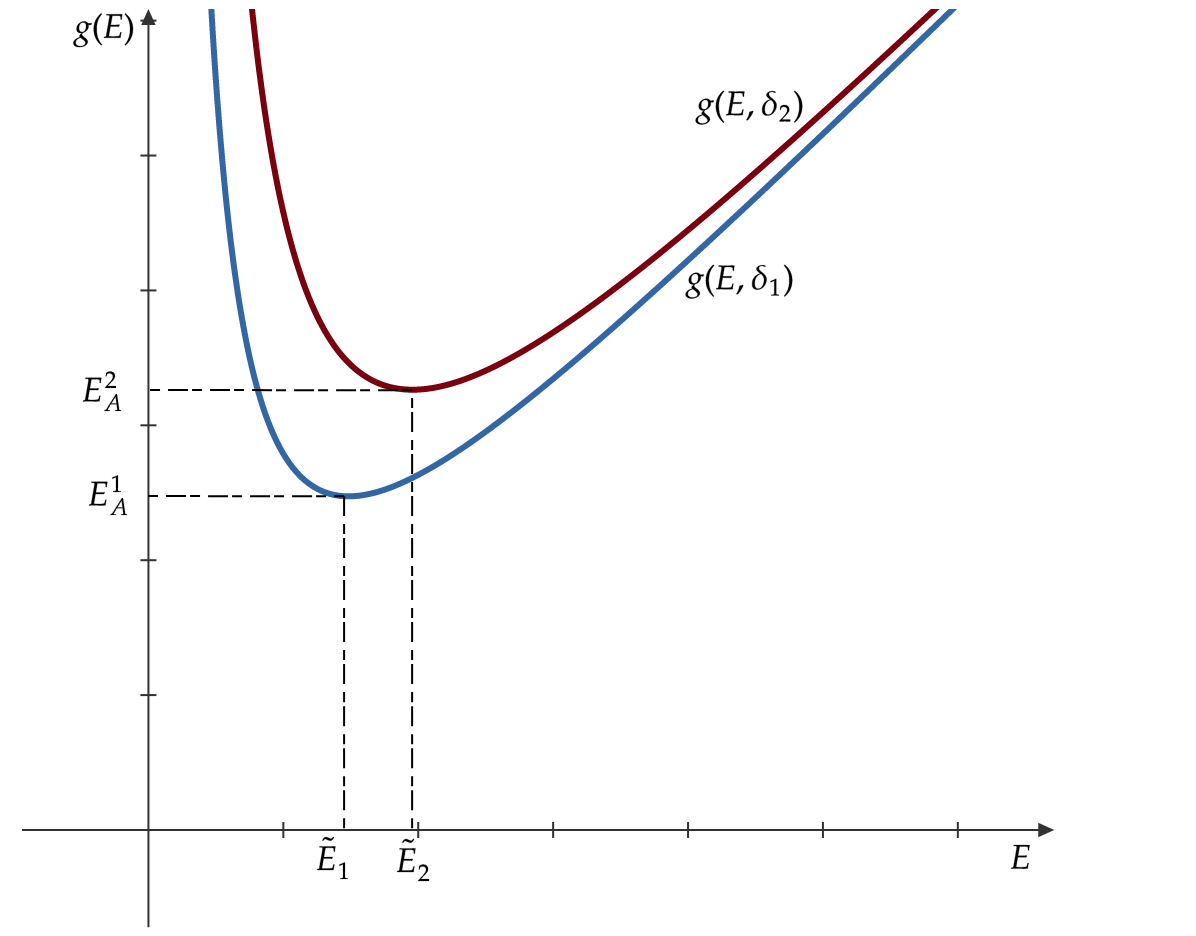
\includegraphics[width=9cm]{graph_g(E).png}
	\caption{The graph of $g(E)$, $E>0$, is drawn for values $\delta_1<\delta_2$ of $\delta$ (clearly in the case of $\alpha+\gamma<1$), when $\delta$ increases then both the coordinates of the minimum point, i.e. $(\tilde{E}, E_A)$ with $E_A=g(\tilde{E})=(\frac{2-2\alpha-\gamma}{1-\alpha-\gamma})\tilde{E}$, increase.}
	\label{fig:graph_g(E)}
\end{figure}

Now, let $P^*=(K^*,E^*,L^*)$ be a stationary state of the system \eqref{eqn:K_dot_E_dot_L_dot} and consider the Jacobian matrix of the same system evaluated at $P^*$
$$
Jac(P^*)=J^* =
\begin{bmatrix}
	0 & 
	0 & 
	\frac{\partial\dot{K}}{\partial L} \\[1ex] % <-- 1ex more space between rows of matrix
	\frac{\partial\dot{E}}{\partial K} & 
	\frac{\partial\dot{E}}{\partial E} & 
	\frac{\partial\dot{E}}{\partial L} \\[1ex]
	\frac{\partial\dot{L}}{\partial K} & 
	\frac{\partial\dot{L}}{\partial E} & 
	\frac{\partial\dot{L}}{\partial L}
\end{bmatrix}
$$
where, by straightforward computations
\begin{equation} \label{eqn:part_deriv_Kdot_Ldot_Edot}
	\begin{split}
		\frac{\partial\dot{K}}{\partial L} &= \frac{\beta+\epsilon}{\delta\epsilon}E^*(\bar{E}-E^*)\\
		\frac{\partial\dot{E}}{\partial K} &=-\delta\theta \\
		\frac{\partial\dot{E}}{\partial E} &=\bar{E}(1-\gamma)-E^*(2-\gamma)\\
		\frac{\partial\dot{E}}{\partial L} &=-(\beta+\epsilon)E^*(\bar{E}-E^*)\\
		\frac{\partial\dot{L}}{\partial K} &=\frac{f(L^*)}{f'(L^*)}\frac{\delta\theta}{E^*} \Bigg[\frac{\theta(1-\alpha)}{\alpha\eta(\bar{E}-E^*)}-\gamma\Bigg]\\
		\frac{\partial\dot{L}}{\partial E} &=\frac{f(L^*)}{f'(L^*)}\frac{\gamma}{E^*} \Bigg[ (1-\gamma)(\bar{E}-E^*)-E^*-\frac{\theta}{\eta} \Bigg]\\
		\frac{\partial\dot{L}}{\partial L} &=\frac{f(L^*)}{f'(L^*)}(\beta+\epsilon) \Bigg[ \frac{\theta(\beta+\epsilon)}{\epsilon}-\frac{\theta}{\eta}-\gamma(\bar{E}-E^*) \Bigg].
	\end{split}
\end{equation}
Another important theorem from the paper holds: 
\begin{thm} \label{thm:num_eigenval_from_Jac}
	If the stationary state is unique with $\alpha+\gamma\geq1$, or, in case of two stationary states, is the one with the larger $E^*$, then $J^*$ has an odd number of positive eigenvalues; instead, if, in case of two stationary states, $P^*$ corresponds to the one with the smaller $E^*$, then $J^*$ has an odd number of negative eigenvalues.
\end{thm}
\begin{proof}
	By computing $det(J^*)$, one can check that
	\begin{equation} \label{eqn:sign_det_J*}
		sign[det(J^*)] = sign[(2-2\alpha-\gamma)E^*-(1-\alpha-\gamma)\bar{E}]
	\end{equation}
	It follows that, when the stationary state is unique and $\alpha+\gamma\geq1$, then $det(J^*) > 0$. Vice versa, when two stationary states exist, implying $\alpha+\gamma<1$, then it follows from \eqref{eqn:sign_det_J*}, by observing Figure \ref{fig:graph_g(E)}, that $det(J^*)$ has the same sign of $g'(E^*)$, which proves the theorem. 
\end{proof}

Considering a non-generic case when a unique stationary state exists under the condition $\alpha+\gamma<1$, then $det(J^*)=0$ holds and the stationary state is not hyperbolic (in fact, a saddle-node bifurcation occurs). Consequently, if one looks for an attracting stationary state, they have to restrict their analysis to the case when, under the assumption $\alpha+\gamma<1$, two stationary states exist, $P_1^*$ and $P_2^*$, with $E_1^* < E_2^*$ and $K_1^* < K_2^*$. Here I aim to show that, in such a context, $P_1^*$ can be attracting for suitable values of the parameters (see Figures \ref{fig:attract_P1_saddle_P2} and \ref{fig:attract_P1_saddle_P2_diff_view}). Along the trajectories belonging to the basin of attraction of $P_1^*$ the over-exploitation of the natural resource drives the economy towards a \textit{tragedy of commons} scenario.
\begin{figure}[h!]
	\centering
	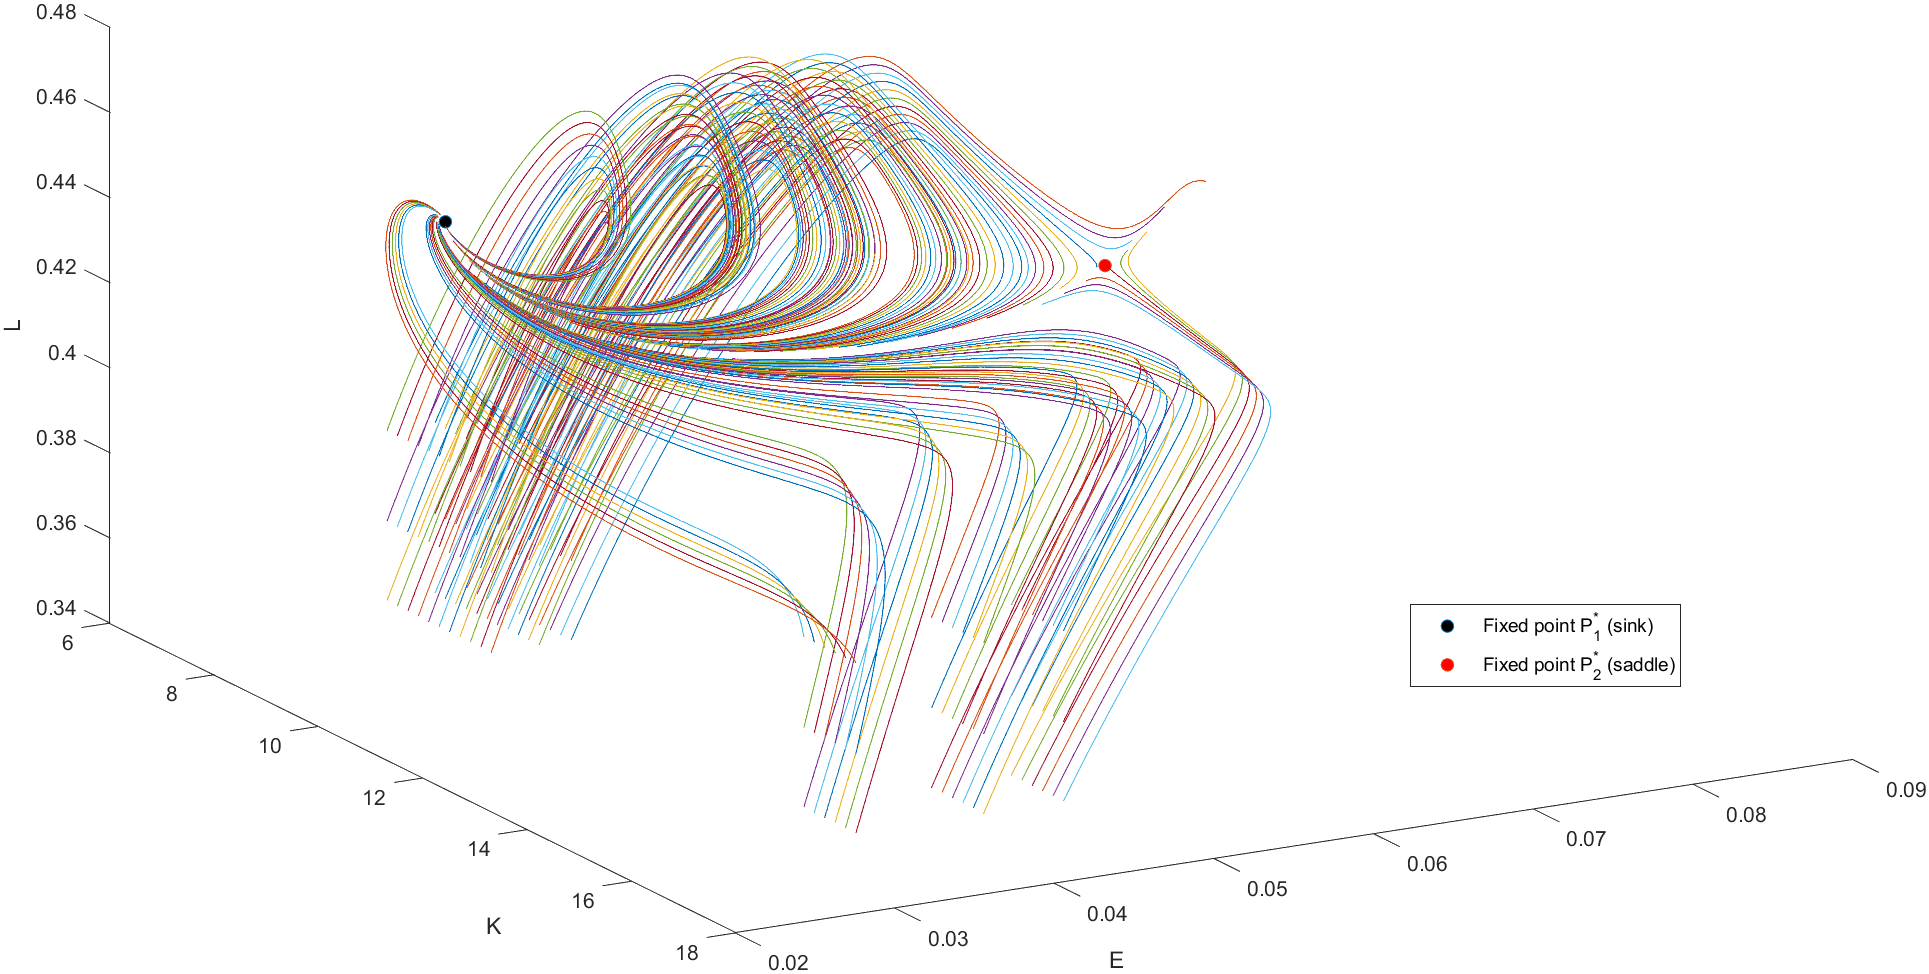
\includegraphics[width=1.\linewidth]{phase_portrait_sink_P1_saddle_P2.png}
	\caption{Phase portrait showing global indeterminacy in the space ($K,E,L$); parameter values: $\alpha=0.1$, $\beta=0.8$, $\gamma=0.58$, $\delta=0.05$, $\epsilon=1$, $\eta=1.5$, $\theta=0.001$, $\bar{E}=0.17$. Considering in particular two trajectories, one approaching the sink $P_1^*=(8.802396759,0.031860545540,0.4444)$ staring from the point ($K_1^*,E_1^*,L_0^1 =0.374591$), while the other approaching the saddle $P_2^*=(13.11009169,0.0591165274446,0.4444)$ starting from the point ($K_1^*,E_1^*,L_0^2 =0.34591$)}
	\label{fig:attract_P1_saddle_P2}
\end{figure}
\begin{figure}[h!]
	\centering
	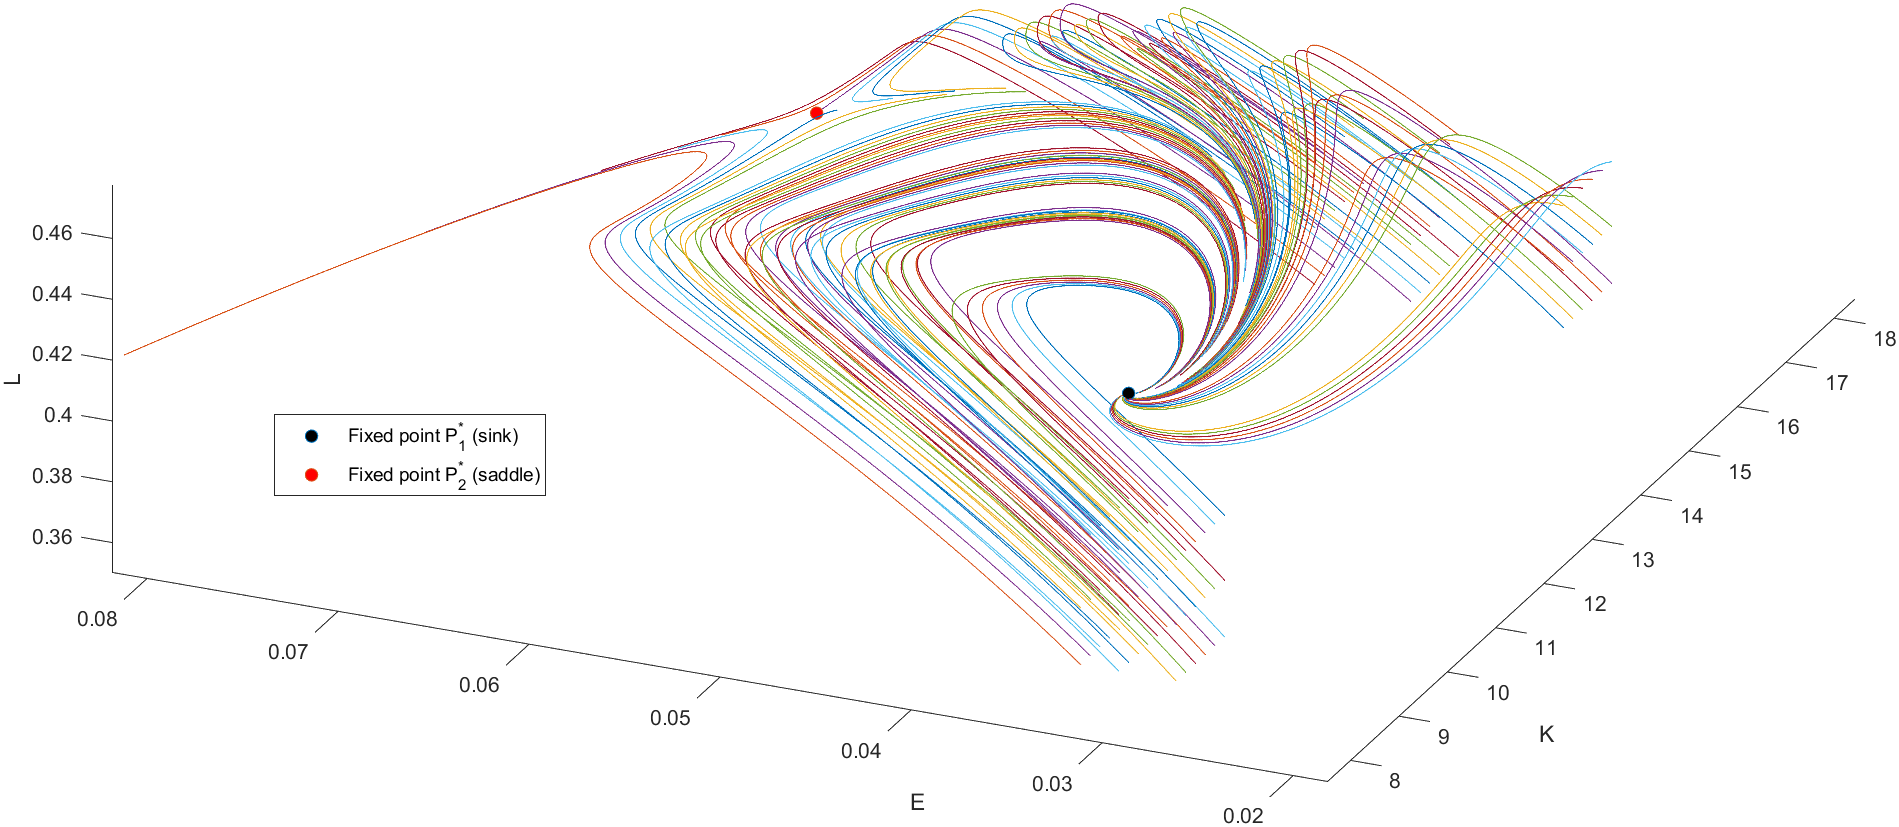
\includegraphics[width=1.\linewidth]{phase_portrait_sink_P1_saddle_P2_bis.png}
	\caption{Different view of the phase portrait.}
	\label{fig:attract_P1_saddle_P2_diff_view}
\end{figure}

First of all, again if $\alpha+\gamma<1$, a necessary and sufficient condition for the existence of two stationary states is
\begin{equation}
	\bar{E}>E_A := g(\tilde{E})=\Bigg(\frac{2-2\alpha-\gamma}{1-\alpha-\gamma}\Bigg) \tilde{E}
\end{equation}
where $\tilde{E}$ is the only positive value satisfying $g'(\tilde{E})=0$. \\
Straightforward computations yield 
\begin{equation} \label{eqn:E_A}
	E_A =(2-2\alpha-\gamma)\Bigg[\frac{\delta^{1-\alpha}}{(1-\alpha)^{1-\alpha}(1-\alpha-\gamma)^{1-\alpha-\gamma}} \Bigg(\frac{\beta}{\beta+\epsilon}\Bigg)^{\beta} \Bigg(\frac{\alpha}{\theta}\Bigg)^{\alpha}\ \Bigg]^{\frac{1}{2-2\alpha-\gamma}}
\end{equation}
Thus, $E_1^*<\tilde{E}<(\frac{1-\alpha-\gamma}{2-2\alpha-\gamma})\bar{E}$.
\underline{From now on the index 1 will be omitted}. 

The well-known Routh–Hurwitz Criterion\footnote{Technique used a lot in control systems which include essentially the calculation of $det(J^*-\lambda I_3)=0$ and derivation of the characteristic equation (in the form of a polynomial). Without calculating directly the eigenvalues of $J^*$, that may be quite complicate in general, one can study only the coefficients of the characteristic equation. Indeed, create the so called Routh table containing the coefficients and a combination of them. Finally, consider some conditions on those terms in the table according to a rule.} (see Hurwitz \cite{hurwitz_conditions_1964}) yields that $J^*$, the Jacobian matrix at $P^*$, has three eigenvalues with negative real part if and only if
\begin{equation} \label{eqn:det_J*_neg}
	det(J^*)<0
\end{equation}
\begin{equation} \label{eqn:cond_sigma_rho_stab}
	\begin{split}
		\sigma(J^*) &= \frac{\partial\dot{E}}{\partial E}\frac{\partial\dot{L}}{\partial L}-\frac{\partial\dot{E}}{\partial L}\frac{\partial\dot{L}}{\partial E}-\frac{\partial\dot{K}}{\partial L}\frac{\partial\dot{L}}{\partial K}>0\\
		\rho(J^*) &= -\sigma(J^*)\cdot trace(J^*)+det(J^*)>0
	\end{split}
\end{equation}
The last inequality, in particular, guarantees the non-existence of complex eigenvalues with non-negative real part. In fact, when $\rho(J^*)$ crosses the origin value $0$, the real part of two complex conjugate eigenvalues changes sign, causing, generically, a Hopf bifurcation.Remember that the condition \eqref{eqn:det_J*_neg} is always verified at $P^*$ (see \eqref{eqn:sign_det_J*}). \\
In fact, as an example, I performed a couple of numerical simulations (the code is available in the appendix \ref{app:A}) using the values of parameters as defined in Figures \ref{fig:attract_P1_saddle_P2} and \ref{fig:local_attract_lim_cycle_P1}, i.e. $\alpha=0.1$, $\beta=0.8$, $\gamma=0.58$, $\delta=0.05$, $\epsilon=1$, $\eta=1.5$, $\theta=0.001$, and with different values of $\bar{E}$.\\
In the first case of the attracting limit cycle with $\bar{E}=0.21$ (hence Hopf bifurcation has already occurred), $\bar{E}>0.167159=E_A$, where $E_A$ comes from \eqref{eqn:E_A}, so one observes two fixed points $P_1^*=(4.5625,0.0115,0.4444)$ and $P_2^*=(21.2463,0.12505,0.4444)$. Considering $P_1^*$ (that is a saddle node with one dimensional stable manifold) and $J^*=Jac(P_1^*)$, I am going to show the conditions coming from the simulation, that are \\$det(J^*)=-2.2387e-07,\quad trace(J^*)=-1.2789e-04,$\\ $\sigma(J^*)=7.1892e-05,\quad \rho(J^*)=-2.1468e-07$. \\
The simulation shows also the three eigenvalues, that are one real negative and the other two complex conjugate with positive real part, and this result is correct since $\rho(J^*)<0$.\\
In the second case (shown in the Figure \ref{fig:attract_P1_saddle_P2}) with the same parameter values but with $\bar{E}=0.17$ one can see again two different fixed points, one a sink and one a saddle. For the sink $P_1^*$ the results are\\ $det(J^*)=-6.5390e-08,\quad trace(J^*)=-0.0237,$\\ $\sigma(J^*)=3.1802e-05,\quad \rho(J^*)=6.8923e-07$,\\ 
with 3 eigenvalues, one real negative and the other two complex conjugate with negative real part. Finally, for the saddle $P_2^*$ the results are\\ $det(J^*)=7.4620e-08,\quad trace(J^*)=-0.0524,$\\ $\sigma(J^*)=7.7007e-07,\quad \rho(J^*)=1.1501e-07$,\\ 
with 3 eigenvalues, two real negative and the third real positive. \\
As for the condition \eqref{eqn:cond_sigma_rho_stab}, the authors of the paper stated the following lemma.
\begin{lemma} \label{lemma:3_condition_for_simga_pos}
	If 
	\begin{equation} \label{eqn:lemma_3}
		\eta\geq \frac{\epsilon}{\epsilon+\alpha\beta} \quad \text{and} \quad \bar{E}>E_B=\frac{\theta(\beta+\epsilon)(2-2\alpha-\gamma)}{\alpha\beta\gamma\eta}
	\end{equation}
	then the condition $\sigma(J^*)>0$ is verified.
\end{lemma}
\begin{proof}
	By recalling \eqref{eqn:part_deriv_Kdot_Ldot_Edot}, straightforward computations lead to 
	$$ sign[\sigma(J^*)] = sign\Bigg[\Bigg(\frac{\beta+\epsilon}{\epsilon}-\frac{1}{\eta}\Bigg)(\bar{E}-2E^*)-\frac{\theta(1-\alpha)(\beta+\epsilon)}{\alpha\epsilon\eta}\Bigg] $$
	So, since $E^*<(\frac{1-\alpha-\gamma}{2-2\alpha-\gamma})\bar{E}$, the assumptions of the lemma imply $\sigma(J^*)>0$.
\end{proof}
I shall now compute $trace(J^*)$; observing that $\frac{f(L^*)}{f'(L^*)}=\frac{\beta\epsilon\eta}{(\beta+\epsilon)[\eta(\beta+\epsilon)-\beta\epsilon]}$, one obtains $$trace(J^*)=a(\bar{E}-E^*)-E^*+b$$ where 

\begin{equation} \label{eqn:a_b_def}
	a:=\frac{\eta[(1-\gamma)(\beta+\epsilon)-\beta\gamma\epsilon]-\beta\epsilon(1-\gamma)}{\eta(\beta+\epsilon)-\beta\epsilon}, \qquad b:=\frac{\beta\theta[\eta(\beta+\epsilon)-\epsilon]}{\eta(\beta+\epsilon)-\beta\epsilon}.
\end{equation}
Then the results from the above analysis, which aim at detecting an attracting stationary state, are summarized by the following theorem.
\begin{thm} \label{thm:result_of_analysis}
	Let $\alpha+\gamma<1$ and $\bar{E}>E_A$, so that system \eqref{eqn:K_dot_E_dot_L_dot} has two stationary states, $P_1^*$ and $P_2^*$, with $E_1^*<E_2^*$ and $K_1^*<K_2^*$. Then there exist values of the parameters for which $P_1^*$ is a sink, while $P_2^*$ is a saddle with a two-dimensional stable manifold. Moreover, in such a case, take $\bar{E}$ as a bifurcation parameter. As $\bar{E}$ is increased, $P_2^*$ does not change its nature (i.e. it remains a saddle with a two-dimensional stable manifold), whereas $P_1^*$ can undergo one, two or no Hopf bifurcations.
\end{thm}
\begin{proof}
	Omitted. See Appendix A of the usual paper \cite{antoci_poverty_2011}.
\end{proof}
Notice that the sufficient conditions for local indeterminacy given above depend on the intertemporal elasticity of substitution\footnote{In economics, intertemporal elasticity of substitution, IES, is a measure of responsiveness of the growth rate of consumption to the real interest rate. For more details see \url{https://en.wikipedia.org/wiki/Elasticity_of_intertemporal_substitution}.} 
and can be satisfied both in case $\eta<1$ (i.e. elasticity of substitution greater than 1) and in case $\eta>1$ (i.e. elasticity of substitution lower than 1): in fact, previously in the lemma they have assumed $\eta\geq \frac{\epsilon}{\epsilon+\alpha\beta}$. Furthermore, those conditions require that the impact of the production process of output (measured by $\delta$) is high enough and/or the subjective discount rate $\theta$ is low enough. Finally, the elasticity $\gamma$ of the production function with respect to the natural capital $E$ must be not too high, that is $\alpha+\gamma<1$, while social returns to scale can be constant or decreasing, that is $\alpha+\beta+\gamma\leq1$.

At this point, the authors have made an analysis about the relation of the coordinates of the fixed points with respect to the parameter $\bar{E}$ (the carrying capacity of the environmental resource). I have performed the numerical simulation fixing the parameters to estimated values, and making sure to have $\alpha+\gamma<1$ (see appendix \ref{app:A}). Figure \ref{fig:plot_K_E_Ebar} shows how the stationary state values of $K$ and $E$ change by varying the value of $\bar{E}$. The coordinates of $P_1^*$ are indicated by a bold line if $P_1^*$ is a sink and by a dash–dot line if it is a saddle with a one-dimensional stable manifold; the coordinates of $P_2^*$ (which, in the numerical example, is a saddle with a two dimensional stable manifold) are indicated by a dotted line. Notice that a Hopf bifurcation occurs when the parameter $\bar{E}$ crosses the value $0.2$ (the bifurcation point is indicated by $H$ or the marker $'*'$ in Figure \ref{fig:plot_K_E_Ebar}).\\
\underline{\bf Remark.} The authors in the paper have also shown the relationship among $K$, $E$ and the parameter $\delta$ (fixing $\bar{E}$), which measure the environmental impact of the production process.\footnote{By observing Figure \ref{fig:graph_g(E)}, it follows that the effect of reducing $\delta$, when $\bar{E}$ is fixed, is qualitatively analogous to that of increasing $\bar{E}$, when $\delta$ is fixed. In fact, as $\delta$ increases, both $\tilde{E}$ and $E_A = g(\tilde{E})$ increase.}
Notice that a Hopf bifurcation occurs also in this example and that indeterminacy is observed when $\delta$ is high enough.
\begin{figure}[h!]
	\centering
	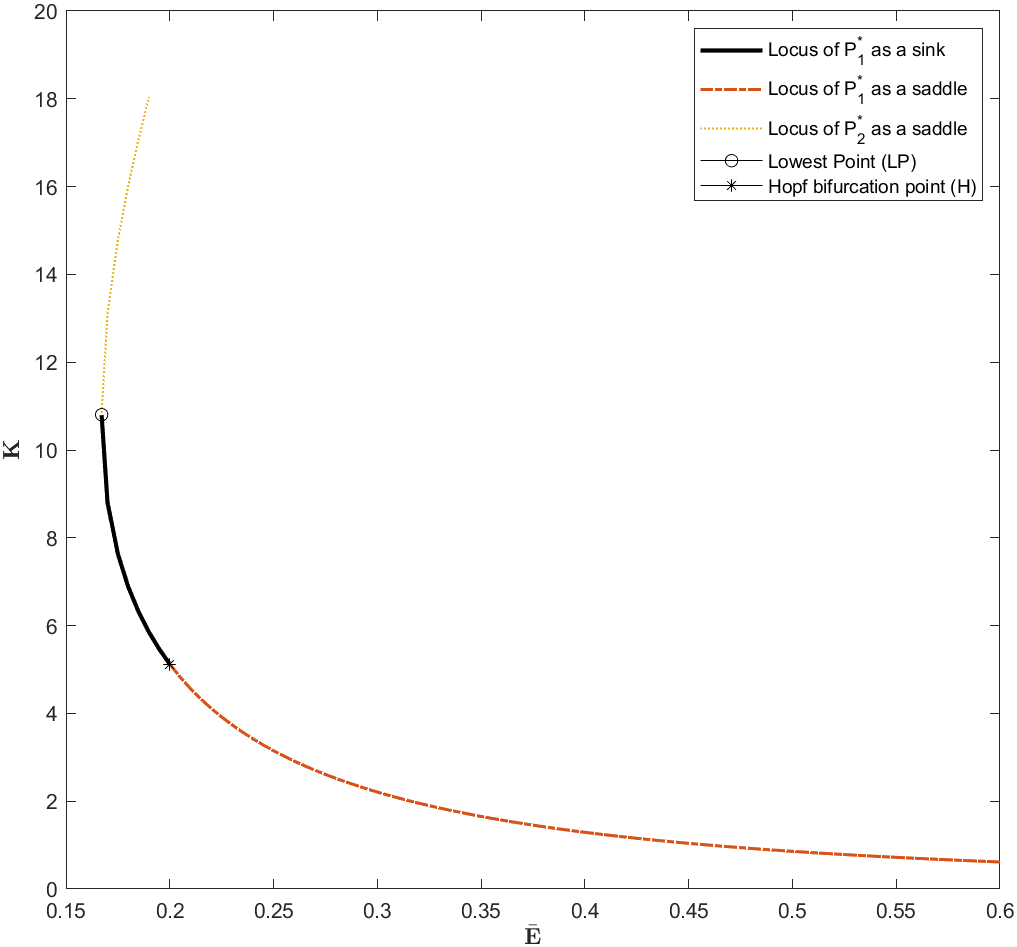
\includegraphics[width=.6\linewidth]{plot_K_Ebar.png}\\
	\vspace{.3cm}
	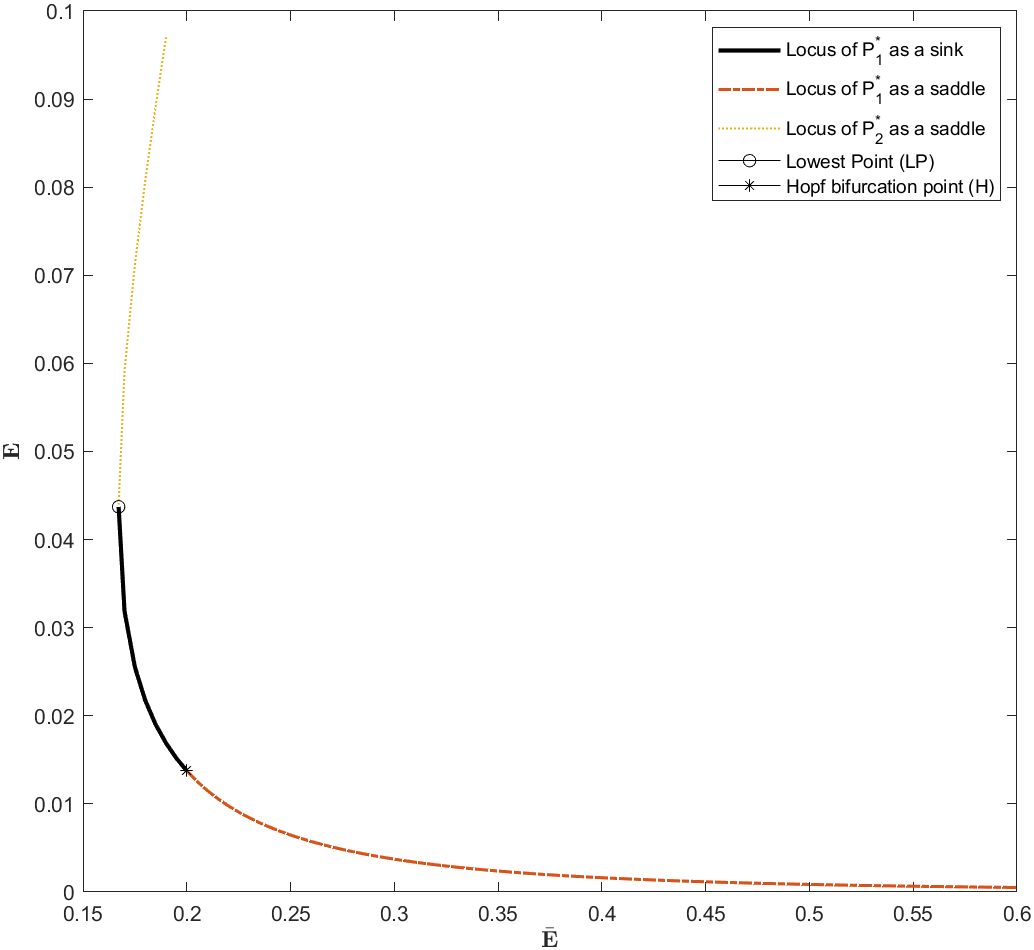
\includegraphics[width=.6\linewidth]{plot_E_Ebar.png}
	\caption{The fixed point values of $K$ and $E$, varying $\bar{E}$; parameter values: $\alpha=0.1$, $\beta=0.8$, $\gamma=0.58$, $\delta=0.05$, $\epsilon=1$, $\eta=1.5$, $\theta=0.001$.}
	\label{fig:plot_K_E_Ebar}
\end{figure}

After performed the numerical simulations of the model using four-stage Runge-Kutta method (see appendix \ref{app:A}), in Figure \ref{fig:local_attract_lim_cycle_P1} is shown a locally attracting limit cycle around $P_1^*$ (which has a one-dimensional stable manifold) arisen via the Hopf bifurcation of Figure \ref{fig:plot_K_E_Ebar}. In such a case (with $\alpha+\gamma<1$), local indeterminacy occurs, since for every initial point $(K_0,E_0)$ close to the projection of the cycle in the plane $(K,E)$, there exists a continuum of initial values $L_0$ of $L$ such that the trajectory starting from $(K_0,E_0,L_0)$ approaches the cycle. In particular, even starting from the fixed point  $P_1^*$ one can observe the attraction to the limit cycle (trajectory in red color in Figure \ref{fig:local_attract_lim_cycle_P1}).
\begin{figure}[h!]
	\centering
	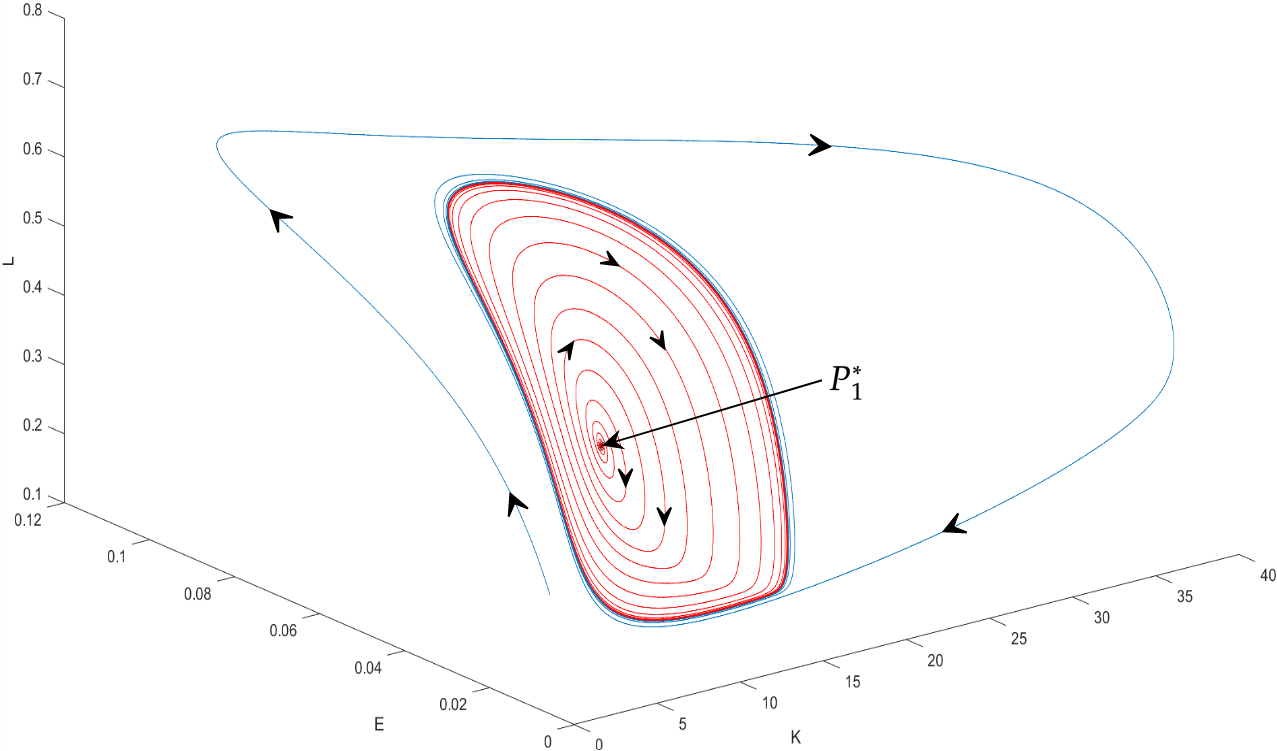
\includegraphics[width=.9\linewidth]{locally_attract_limit_cycle_fixPnt_P1.png}
	\caption{Locally attracting limit cycle "around" $P_1^*$; parameter values: $\alpha=0.1$, $\beta=0.8$, $\gamma=0.58$, $\delta=0.05$, $\epsilon=1$, $\eta=1.5$, $\theta=0.001$.}
	\label{fig:local_attract_lim_cycle_P1}
\end{figure}

Now to complete the local analysis I shall discuss the case $\alpha+\gamma>1$, when the stationary state $P^*$ is unique. Since $det(J^*) > 0$ (see Theorem \ref{thm:num_eigenval_from_Jac}), $P^*$ is not attracting. If, for some value of $\bar{E}$, $trace(J^*)=a(\bar{E}-E^*)-E^*+b<0$, with $a$ and $b$ defined in \eqref{eqn:a_b_def}, then $P^*$ is a saddle with a two-dimensional stable manifold. By the equilibrium condition $g(E^*)=\bar{E}$, one can write $trace(J^*)$ as
$$trace(J^*)=r(E^*)^{\frac{\alpha+\gamma-1}{1-\alpha}}-E^*+b$$
with $b>0$, $\alpha+\gamma-1>0$ and $sign(r)=sign(a)$. 
By the same arguments developed in Theorem \ref{thm:result_of_analysis}, the following one is easily proved.
\begin{thm} \label{thm:5_no_indeter_with_unique_fixPnt}
	Let $\alpha+\gamma>1$ and $P^*$ denote the only stationary state of system \eqref{eqn:K_dot_E_dot_L_dot}. Write $trace(J^*)=a(\bar{E}-E^*)-E^*+b$, with $a$ and $b$ defined in \eqref{eqn:a_b_def}. Assume $trace(J^*) < 0$ for some value of $\bar{E}$ and let $\bar{E}$ increase. Then: if $a\leq0$, no bifurcation occurs and $P^*$ remains a saddle with a two-dimensional stable manifold; if $a>0$ and $2\alpha+\gamma>2$, eventually $P^*$ becomes a source and one Hopf bifurcation generically takes place; if $a>0$ and $2\alpha+\gamma<2$, $P^*$ is a saddle with a two-dimensional stable manifold for sufficiently large values of $\bar{E}$ and Hopf bifurcations are, generically, zero or two.
\end{thm}
According to the above theorem, indeterminacy cannot be observed in the context of a unique stationary state: i.e., the stationary state can possess saddle-type stability (two eigenvalues with negative real part) but cannot be a sink.